\documentclass{standalone}
\usepackage{tikz}
\usetikzlibrary{patterns, positioning}


\begin{document}
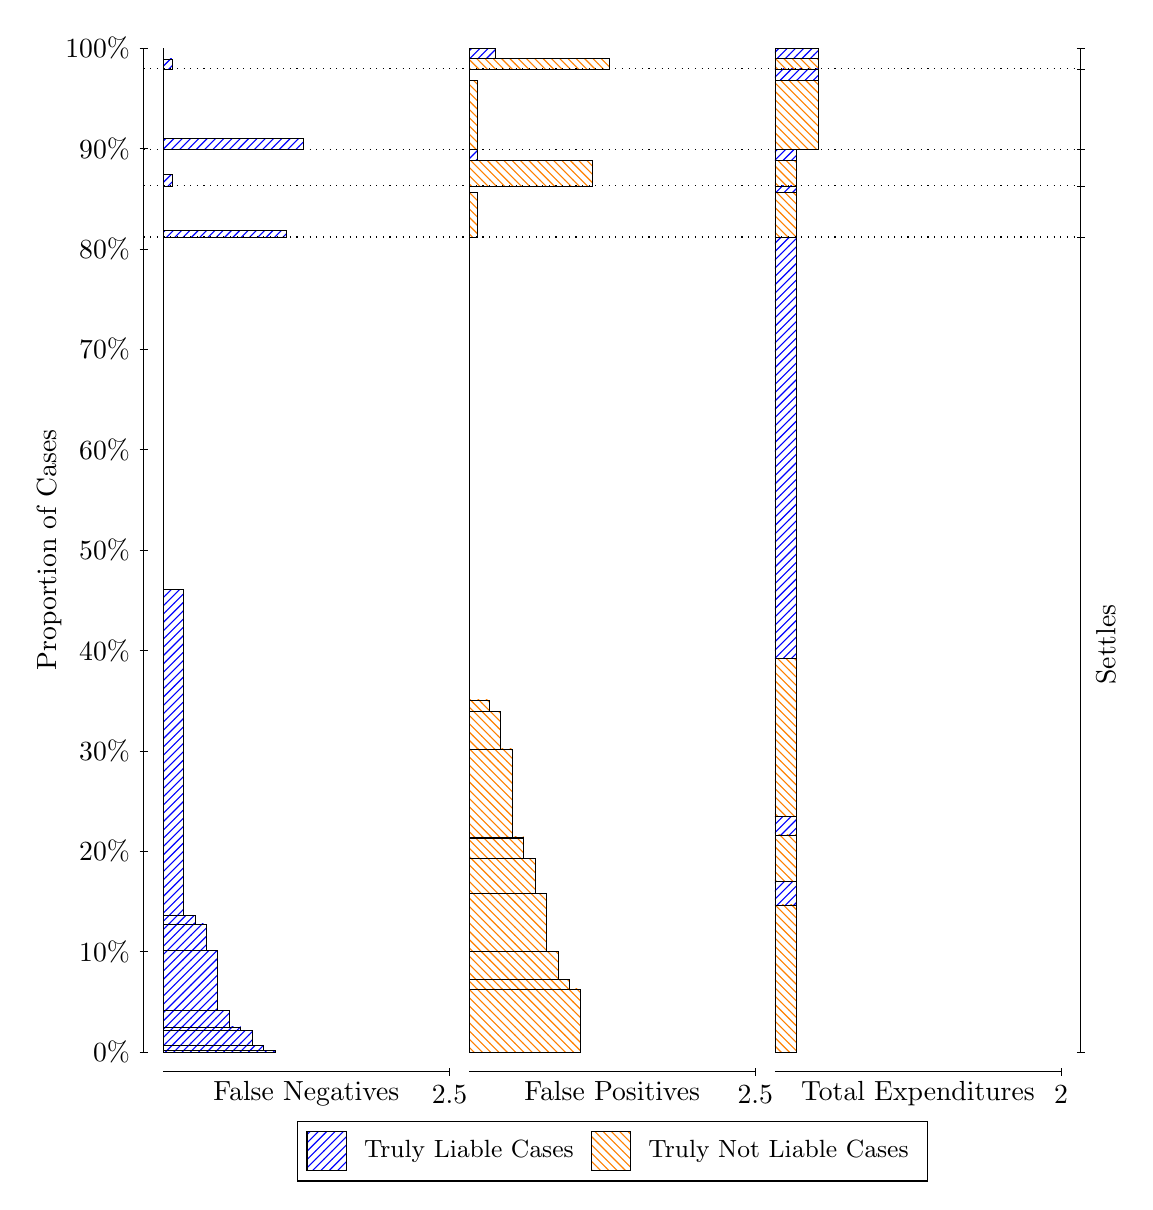
\begin{tikzpicture}
\draw[black, very thin] (1.5,1.75) -- (1.5,14.5);
\node[rotate=90, text=black, anchor=center] at (0.3, 8.125) {Proportion of Cases};
\draw[black, very thin] (1.45,1.75) -- (1.55,1.75);
\node[text=black, anchor=east] at (1.45, 1.75) {0\%};
\draw[black, very thin] (1.45,3.025) -- (1.55,3.025);
\node[text=black, anchor=east] at (1.45, 3.025) {10\%};
\draw[black, very thin] (1.45,4.3) -- (1.55,4.3);
\node[text=black, anchor=east] at (1.45, 4.3) {20\%};
\draw[black, very thin] (1.45,5.575) -- (1.55,5.575);
\node[text=black, anchor=east] at (1.45, 5.575) {30\%};
\draw[black, very thin] (1.45,6.85) -- (1.55,6.85);
\node[text=black, anchor=east] at (1.45, 6.85) {40\%};
\draw[black, very thin] (1.45,8.125) -- (1.55,8.125);
\node[text=black, anchor=east] at (1.45, 8.125) {50\%};
\draw[black, very thin] (1.45,9.4) -- (1.55,9.4);
\node[text=black, anchor=east] at (1.45, 9.4) {60\%};
\draw[black, very thin] (1.45,10.675) -- (1.55,10.675);
\node[text=black, anchor=east] at (1.45, 10.675) {70\%};
\draw[black, very thin] (1.45,11.95) -- (1.55,11.95);
\node[text=black, anchor=east] at (1.45, 11.95) {80\%};
\draw[black, very thin] (1.45,13.225) -- (1.55,13.225);
\node[text=black, anchor=east] at (1.45, 13.225) {90\%};
\draw[black, very thin] (1.45,14.5) -- (1.55,14.5);
\node[text=black, anchor=east] at (1.45, 14.5) {100\%};

\draw[black, very thin] (13.4,1.75) -- (13.4,14.5);
\draw[black, very thin] (13.35,1.75) -- (13.45,1.75);
\node[anchor=west] at (13.35, 1.75) {};
\draw[black, very thin] (13.35,12.1) -- (13.45,12.1);
\node[anchor=west] at (13.35, 12.1) {};
\draw[black, very thin] (13.35,12.749) -- (13.45,12.749);
\node[anchor=west] at (13.35, 12.749) {};
\draw[black, very thin] (13.35,13.215) -- (13.45,13.215);
\node[anchor=west] at (13.35, 13.215) {};
\draw[black, very thin] (13.35,14.235) -- (13.45,14.235);
\node[anchor=west] at (13.35, 14.235) {};
\draw[black, very thin] (13.35,14.5) -- (13.45,14.5);
\node[anchor=west] at (13.35, 14.5) {};

\draw[black, very thin, pattern color=blue, pattern=north east lines] (1.75,1.75) rectangle (3.167,1.7691);
\draw[black, very thin, pattern color=blue, pattern=north east lines] (1.75,1.7691) rectangle (3.0217,1.8333);
\draw[black, very thin, pattern color=blue, pattern=north east lines] (1.75,1.8333) rectangle (2.8763,2.0228);
\draw[black, very thin, pattern color=blue, pattern=north east lines] (1.75,2.0228) rectangle (2.731,2.0676);
\draw[black, very thin, pattern color=blue, pattern=north east lines] (1.75,2.0676) rectangle (2.5857,2.2807);
\draw[black, very thin, pattern color=blue, pattern=north east lines] (1.75,2.2807) rectangle (2.4403,3.0438);
\draw[black, very thin, pattern color=blue, pattern=north east lines] (1.75,3.0438) rectangle (2.295,3.3765);
\draw[black, very thin, pattern color=blue, pattern=north east lines] (1.75,3.3765) rectangle (2.1497,3.4883);
\draw[black, very thin, pattern color=blue, pattern=north east lines] (1.75,3.4883) rectangle (2.0043,7.6288);
\draw[black, very thin, pattern color=orange, pattern=north west lines] (1.75,7.6288) rectangle (1.75,12.1);
\draw[black, very thin, pattern color=blue, pattern=north east lines] (1.75,12.1) rectangle (3.3123,12.181);
\draw[black, very thin, pattern color=orange, pattern=north west lines] (1.75,12.181) rectangle (1.75,12.749);
\draw[black, very thin, pattern color=blue, pattern=north east lines] (1.75,12.749) rectangle (1.859,12.895);
\draw[black, very thin, pattern color=orange, pattern=north west lines] (1.75,12.895) rectangle (1.75,13.215);
\draw[black, very thin, pattern color=blue, pattern=north east lines] (1.75,13.215) rectangle (3.5303,13.357);
\draw[black, very thin, pattern color=orange, pattern=north west lines] (1.75,13.357) rectangle (1.75,14.235);
\draw[black, very thin, pattern color=blue, pattern=north east lines] (1.75,14.235) rectangle (1.859,14.362);
\draw[black, very thin, pattern color=orange, pattern=north west lines] (1.75,14.362) rectangle (1.75,14.5);
\draw[black, very thin, pattern color=orange, pattern=north west lines] (5.6333,1.75) rectangle (7.0503,2.5503);
\draw[black, very thin, pattern color=orange, pattern=north west lines] (5.6333,2.5503) rectangle (6.905,2.6759);
\draw[black, very thin, pattern color=orange, pattern=north west lines] (5.6333,2.6759) rectangle (6.7597,3.0296);
\draw[black, very thin, pattern color=orange, pattern=north west lines] (5.6333,3.0296) rectangle (6.6143,3.7638);
\draw[black, very thin, pattern color=orange, pattern=north west lines] (5.6333,3.7638) rectangle (6.469,4.2038);
\draw[black, very thin, pattern color=orange, pattern=north west lines] (5.6333,4.2038) rectangle (6.3237,4.4671);
\draw[black, very thin, pattern color=orange, pattern=north west lines] (5.6333,4.4671) rectangle (6.3237,4.4826);
\draw[black, very thin, pattern color=orange, pattern=north west lines] (5.6333,4.4826) rectangle (6.1783,5.5996);
\draw[black, very thin, pattern color=orange, pattern=north west lines] (5.6333,5.5996) rectangle (6.033,6.0713);
\draw[black, very thin, pattern color=orange, pattern=north west lines] (5.6333,6.0713) rectangle (5.8877,6.2214);
\draw[black, very thin, pattern color=blue, pattern=north east lines] (5.6333,6.2214) rectangle (5.6333,12.1);
\draw[black, very thin, pattern color=orange, pattern=north west lines] (5.6333,12.1) rectangle (5.7423,12.668);
\draw[black, very thin, pattern color=blue, pattern=north east lines] (5.6333,12.668) rectangle (5.6333,12.749);
\draw[black, very thin, pattern color=orange, pattern=north west lines] (5.6333,12.749) rectangle (7.1957,13.069);
\draw[black, very thin, pattern color=blue, pattern=north east lines] (5.6333,13.069) rectangle (5.7423,13.215);
\draw[black, very thin, pattern color=orange, pattern=north west lines] (5.6333,13.215) rectangle (5.7423,14.093);
\draw[black, very thin, pattern color=blue, pattern=north east lines] (5.6333,14.093) rectangle (5.6333,14.235);
\draw[black, very thin, pattern color=orange, pattern=north west lines] (5.6333,14.235) rectangle (7.4137,14.373);
\draw[black, very thin, pattern color=blue, pattern=north east lines] (5.6333,14.373) rectangle (5.9603,14.5);
\draw[black, very thin, pattern color=orange, pattern=north west lines] (9.5167,1.75) rectangle (9.7892,3.6175);
\draw[black, very thin, pattern color=blue, pattern=north east lines] (9.5167,3.6175) rectangle (9.7892,3.916);
\draw[black, very thin, pattern color=orange, pattern=north west lines] (9.5167,3.916) rectangle (9.7892,4.5062);
\draw[black, very thin, pattern color=blue, pattern=north east lines] (9.5167,4.5062) rectangle (9.7892,4.7383);
\draw[black, very thin, pattern color=orange, pattern=north west lines] (9.5167,4.7383) rectangle (9.7892,6.7521);
\draw[black, very thin, pattern color=blue, pattern=north east lines] (9.5167,6.7521) rectangle (9.7892,12.1);
\draw[black, very thin, pattern color=orange, pattern=north west lines] (9.5167,12.1) rectangle (9.7892,12.668);
\draw[black, very thin, pattern color=blue, pattern=north east lines] (9.5167,12.668) rectangle (9.7892,12.749);
\draw[black, very thin, pattern color=orange, pattern=north west lines] (9.5167,12.749) rectangle (9.7892,13.069);
\draw[black, very thin, pattern color=blue, pattern=north east lines] (9.5167,13.069) rectangle (9.7892,13.215);
\draw[black, very thin, pattern color=orange, pattern=north west lines] (9.5167,13.215) rectangle (10.062,14.093);
\draw[black, very thin, pattern color=blue, pattern=north east lines] (9.5167,14.093) rectangle (10.062,14.235);
\draw[black, very thin, pattern color=orange, pattern=north west lines] (9.5167,14.235) rectangle (10.062,14.373);
\draw[black, very thin, pattern color=blue, pattern=north east lines] (9.5167,14.373) rectangle (10.062,14.5);
\draw[black, dotted] (1.5,12.1) -- (13.4,12.1);
\draw[black, dotted] (1.5,12.749) -- (13.4,12.749);
\draw[black, dotted] (1.5,13.215) -- (13.4,13.215);
\draw[black, dotted] (1.5,14.235) -- (13.4,14.235);
\draw[black, very thin] (1.75,1.5) -- (5.3833,1.5);
\node[text=black, anchor=north] at (3.5667, 1.5) {False Negatives};
\draw[black, very thin] (5.3833,1.45) -- (5.3833,1.55);
\node[text=black, anchor=north] at (5.3833, 1.45) {2.5};

\draw[black, very thin] (5.6333,1.5) -- (9.2667,1.5);
\node[text=black, anchor=north] at (7.45, 1.5) {False Positives};
\draw[black, very thin] (9.2667,1.45) -- (9.2667,1.55);
\node[text=black, anchor=north] at (9.2667, 1.45) {2.5};

\draw[black, very thin] (9.5167,1.5) -- (13.15,1.5);
\node[text=black, anchor=north] at (11.333, 1.5) {Total Expenditures};
\draw[black, very thin] (13.15,1.45) -- (13.15,1.55);
\node[text=black, anchor=north] at (13.15, 1.45) {2};

\node[text=black, centered, rotate=90] at (13.72, 6.9251) {Settles};





\draw (7.449999999999999,1.5) node[draw=none] (baseCoordinate) {};
\begin{scope}[align=center]
        \matrix[scale=0.5, draw=black, below=0.5cm of baseCoordinate, nodes={draw}, column sep=0.1cm]{
            \node[rectangle, draw, minimum width=0.5cm, minimum height=0.5cm, pattern color=blue, pattern=north east lines] {}; &
            \node[draw=none, font=\small, text=black] (B) {Truly Liable Cases}; &
            \node[rectangle, draw, minimum width=0.5cm, minimum height=0.5cm, pattern color=orange, pattern=north west lines] {}; &
            \node[draw=none, font=\small, text=black] (B) {Truly Not Liable Cases}; \\
            };
\end{scope}

\end{tikzpicture}
\end{document}